\newgeometry{top=3cm, bottom=2cm}
\chapter{Results}
\label{chapter:results}

This chapter covers the results and analysis of the case study. First the results of interview for demographic purposes are
presented. Second, survey and interview results regarding JUnit compared to Spock and Spectrum are analyzed.  Third, the test
code analysis is presented and finally
with all the above mentioned results, Spock and Spectrum are compared against each other.


%-Define the population to which inferential statistics and predictive models apply.\newline
%-RQ1 and RQ2 answered by comparing initial and post surveys\newline
%-Comparing Spock and Spectrum vs each other\newline
%-RQ3 answered by comparing observed actual test implementation changes\newline

\section{First interview: Demographics and projects}
\label{section:demographics}
    First interview was conducted to study about the demographics of participants and projects under research.
    The demographics of participants are displayed in table \ref{tab:demographics}. To summarize the
    participants, all can be categorized as senior software developers with many years of working with \textit{xUnit testing family} frameworks.
    Only participant C has a fair amount of prior experience working with BDD testing frameworks.
    \begin{table}[H]
        \resizebox{\textwidth}{!}{%
            \begin{tabular}{p{8.0cm}*{3}{p{3.5cm}}}
            \headcol & & &  \\
            \headcol {\large\textbf{Participant attribute}} & {\large\textbf{Participant A}} & {\large\textbf{Participant B}} & {\large\textbf{Participant C}} \\
            \hline
            \rowcol & & & \\
            \rowcol \textbf{Project} & Project A & Project A & Project B \\ \hline
            & & & \\
            \textbf{Software development experience} & 17 years & 15 years & 8 years \\ \hline
            \rowcol & & &  \\
            \rowcol \textbf{Java development experience} & 14 years & 1 year & 5-6 years  \\ \hline
            & & &  \\
            \textbf{Spring Framework experience} & 7 years & 1 year & 5-6 years \\ \hline
            \rowcol & & &  \\
            \rowcol \textbf{Automated unit testing experience} & 14 years; & 10 years; & 3-4 years; \\
            \rowcol \multicolumn{1}{r}{\textit{with frameworks}\textcolor{white}{-------------}} & \textit{JUnit} & \textit{CPPUnit, JUnit} & \textit{JUnit, TestNG} \\ \hline
            & & &  \\
            \textbf{Automated integration testing \newline experience} & 14 years; & Hardly at all; & 5-6 years; \\
            \multicolumn{1}{r}{\textit{with frameworks}\textcolor{white}{------------}} & \textit{JUnit, Some Robot Framework with Selenium} & \textit{JUnit} & \textit{JUnit, TestNG} \\ \hline
            \rowcol & & &  \\
            \rowcol \textbf{BDD testing framework experience} & \textless \textit{ } 1 year; & - & 2-3 years; \\
            \rowcol \multicolumn{1}{r}{\textit{with frameworks}\textcolor{white}{------------}} & \textit{Jasmine, Mocha} & & \textit{JBehave} \\
            \rowcol & & &  \\ \bottomlinec
            \end{tabular}}
            \caption {Participant demographics} \label{tab:demographics}
    \end{table}
\restoregeometry

The projects under study can both be categorized as web application projects with Java \textit{Spring Framework} backend technology.
They both have an agile development process. \textbf{Project A} is a customer project in public administration context.
\textbf{Project B} is an in-house project. They are both on the medium scale in code size, but financially project A can be
categorized as medium to large category.

Project A has two developers, \textbf{participants A} and \textbf{B}, working with Spring Framework backend,
where there is automated low-level testing in place with \textit{JUnit}.
Project B has only one backend developer, \textbf{participant C}, working with Spring Framework. As Project B
was developed in larger scale from 2012 to 2013 and published originally in 2013, it has some of the automated
low-level testing with JUnit done by others than participant C. Still most of this kind of test work is done by participant C.
Table \ref{tab:projects} displays the details of projects A and B.
    \begin{table}[H]
        \resizebox{\textwidth}{!}{%
            \begin{tabular}{p{7.5cm}*{2}{p{6cm}}}
            \headcol & & \\
            \headcol {\large\textbf{Project attribute}} & {\large\textbf{Project A}} & {\large\textbf{Project B}} \\ \hline
            \rowcol & &  \\
            \rowcol \textbf{Description} & Web application for area management, replacing existing system & Wep application for working hours tracking \& reporting \\ \hline
            & &   \\
            \textbf{Context} & Public administration, development for customer & In-house develoment \\ \hline
            \rowcol & & \\
            \rowcol \textbf{Development process} & Agile development with customized \textit{Scrum} & Agile with loosely defined process \\ \hline
            & &  \\
            \textbf{Size \& development team} & Medium - large project; \newline 3 developers for approximately 1,5 years & Small - medium project; \newline Published 2013, now 2 developers maintaining \& further development \\ \hline
            \rowcol & & \\
            \rowcol \textbf{Architecture} & Client rendered single-page \newline application & Server MVC with some client rendered views \\ \hline
            & & \\
            \textbf{Technologies} & \textit{Java Spring Boot \& Angular 2} & \textit{Java Spring Framework \& JSP, Backbone.js} \\ \hline
            \rowcol & & \\
            \rowcol \textbf{Quality assurance process} & Automated unit \& integration testing, code reviews, continuous integration, no dedicated tester & Automated unit, integration \& acceptance testing, code reviews, continuous integration, no dedicated tester \\ \hline
            & & \\
            \textbf{Used unit testing framework} & \textit{JUnit} & \textit{JUnit} \\ \hline
            \rowcol & &  \\
            \rowcol \textbf{Used integration testing framework} & \textit{JUnit} extended for \textit{Spring Framework} & \textit{JUnit} extended for \textit{Spring Framework} \\\hline
            \textbf{Chosen BDD testing framework} & \textit{Spectrum} & \textit{Spock} \\
            & &  \\ \bottomlinec
            \end{tabular}}
            \caption {Project details} \label{tab:projects}
    \end{table}

\section{Surveys and BDD framework feedback interview analyzed}
This section covers the results analyzed for both JUnit and BDD framework surveys together with participant BDD framework feedback interviews.
First the developer practices and their changes are answered with the data. Second, developer perception of low-level
testing and its changes are illustrated. Together these sections answer RQ1 \& and RQ2.

The baseline for answers was conducted with the survey described in detail in Appendix \ref{chapter:surveys} section \ref{section:junit-survey}.
These questions related to JUnit low-level testing are displayed with \textbf{Q1, Q2, Q3} and so on. Their counterparts, questions aimed to study the changes
in low-level testing with new BDD implementation level testing framework are marked as \textbf{Q1', Q2', Q3'} and so on. Details
of BDD surveys can be found in Appendix \ref{chapter:surveys} section \ref{section:bdd-survey}. Participants whom answered
the surveys were {\colorbox{lightgray}A}, {\colorbox{lime}B} and {\colorbox{orange}C}. The color coding of participants is
visible throughout the result tables for easier highlighting of answers.

\subsection{Automated low-level testing developer practices}
This section answer the
\textbf{RQ1: }\textit{How does behavior driven testing frameworks change developer practices working with automated
low-level testing compared to JUnit framework?} This is studied through multiple aspects, which all display results and analysis
individually. First, the developer software development \& testing time and effort usage is analyzed. Second, low-level
test optimizing targets are inspected. Third, test understandability and informativiness is under study. After that, test
refactoring techniques and commenting practices are analyzed. Finally, unit testing practices are studied in more detail
before summarizing the answers to RQ1 and the changes in low-level testing developer practices.

\subsubsection{Software development \& testing time and effort usage}
    \begin{figure}[ht]%
        \centering
        \subfloat[Results in original study~\cite{daka2014survey} ]{{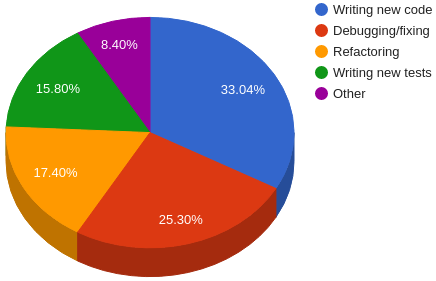
\includegraphics[width=6.75cm]{images/org-time.png} }}%
        \qquad
        \subfloat[Results in this study]{{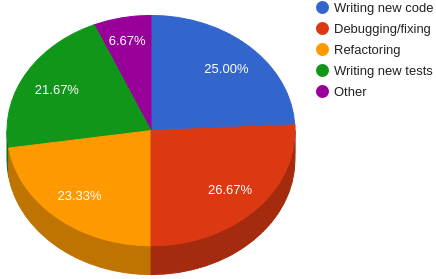
\includegraphics[width=6.75cm]{images/new-time.png} }}%
        \caption{Developer software development time usage}%
        \label{fig:time-usage}%
    \end{figure}
First studied aspect of developer practices was \textbf{time usage}. Figure \ref{fig:time-usage} displays the developer software development time usage
in original study~\cite{daka2014survey} and in this thesis. Table \ref{tab:changes-pt1a} display the participant values
also individually and the changes in time usage after the introduction of a new BDD framework. In the original study, writing
new code is the dominating activity in time usage with 33.04\% share. At the beginning of this study when studying JUnit practices,
participants used most of their software development
time in \textit{debugging or fixing} activities with 26.67\% time usage share. \textit{Writing new code} (25.00\%) and \textit{refactoring} (23.33\%) were close
by in time usage. The participants in this study had quite much variance in their answers for time usage, but \textit{writing
new tests} was uniformly higher in time usage than in the original study results. Participants {\colorbox{lightgray}A} and {\colorbox{orange}C}
were closely together in their answers for time usage, whereas participant {\colorbox{lime}B} had more emphasis on initial \textit{writing of new code} and
less time spent on \textit{refactoring}.

    \begin{table}[H]
        \resizebox{\textwidth}{!}{%
            \begin{tabular}{p{13.0cm}*{7}{p{2cm}}}
            \topline
            \textbf{Question} & \textbf{Answer options} &  &  &  &   &  & \\ \hline
            \textbf{Q1: How do you spend your software development time (in percentages)} & Participant {\colorbox{lightgray}A} & Participant {\colorbox{lime}B} & Participant {\colorbox{orange}C} & Average & & \\
            & & & & & & & \\
            1. Writing new code & 20\% & 40\% & 15\% & 25\%  \\
            2. Writing new tests & 20\% & 25\% & 20\% & 21.67\% \\
            3. Debugging/fixing & 30\% & 25\% & 25\% & 26.67\% \\
            4. Refactoring & 20\%  & 10\% & 30\% & 23.33\% \\
            5. Other & 10\% & 0\% & 10\% & 6.67\% \\
            & \\ \hline
            \textbf{Q1': Compared to JUnit, How do you spend your software development time?} & A lot less time & Less time & Slightly less time & The Same amount of time & Slightly more time & More time & A lot more time \\
            & \\
            1. Writing new code & 0 & 0 & 0 & {\colorbox{lightgray}A} & 0 & 0 & 0 \\
            2. Writing new tests & 0 & 0 & 0 & {\colorbox{lightgray}A} & 0 & 0 & 0 \\
            3. Debugging/fixing & 0 & 0 & 0 & {\colorbox{lightgray}A} & 0 & 0 & 0 \\
            4. Refactoring & 0 & 0 & 0 & {\colorbox{lightgray}A} & 0 & 0 & 0 \\
            5. Other & 0 & 0 & 0 & {\colorbox{lightgray}A} & 0 & 0 & 0 \\
            & \\ \topline


            \end{tabular}}
            \caption {Development time usage and changes in it} \label{tab:changes-pt1a}
    \end{table}

Changes in software development time were studied with the \textbf{Q1':} \textit{Compared to JUnit, How do you spend your
software development time?} Results are displayed in table \ref{tab:changes-pt1a}. Participant {\colorbox{lightgray}A}
didn't see any changes in the overall software development time usages after introduction of \textbf{\textit{Spectrum}}. This has to be taken
with a grain of salt, as the  next questions shows increase in testing efforts when comparing JUnit and Spectrum.

\textbf{TO BE CONTINUED}

\clearpage

Questions \textbf{Q2} and \textbf{Q2'} further analyze the time usage, now focusing in automated testing. Their results are
shown in table \ref{tab:changes-pt1b}. All participants answered to use approximately 30 minutes of time in single test case. The
averages show that about one third (28.33\%) of initial effort goes to \textit{thinking} about the test case without actual implementation.
About two thirds (71.67\%) of initial effort goes to \textit{implementation} of the test case. \textit{Refactoring} takes about one third (28.33\%)
of the overall testing effort.

Participants had highly varying answers in initial \textit{thinking} and \textit{implementation} effort and also
in overall testing \textit{refactoring} effort. Participants {\colorbox{lime}B} and {\colorbox{orange}C} had same kind of profile
in initial efforts, where about one fifth of it goes to initial \textit{thinking} of test case and four fifths to \textit{implementation}.
Participant {\colorbox{lightgray}A} had the initial effort going in half between the two aspects. In overall effort,
\textit{refactoring} of test code took 50\% of effort for participant {\colorbox{lightgray}A}. Participant {\colorbox{lime}B}
hardly at all \textit{refactored} test code (5\%) and participant {\colorbox{orange}C} used around one third of overall testing effort
to \textit{refactoring} (30\%).


    \begin{table}[H]
        \resizebox{\textwidth}{!}{%
            \begin{tabular}{p{13.0cm}*{7}{p{2cm}}}
            \topline
            \textbf{Question} & \textbf{Answer options} &  &  &  &   &  & \\ \hline
            \textbf{Q2: How do you spend your low-level automated testing time} & Participant {\colorbox{lightgray}A} & Participant {\colorbox{lime}B} & Participant {\colorbox{orange}C} & Average & & \
            & & & & & & & \\
            1. How much approximately you use time per test case (minutes)? & 30 min & 30 min & 30 min & 30 min \\
            2. How much of your initial effort goes to thinking about test case content without implementation (percentage)? & 50\% & 20\% & 15\% & 28.33\% \\
            3. How much of your initial effort goes to initial test case structuring and implementation (percentage)? & 50\% & 80\% & 85\% & 71.67\% \\
            4. How much of your overall testing effort goes to refactoring test code (percentage)? & 50\% & 5\% & 30\% & 28.33\% \\
            & \\ \hline
            \textbf{Q2': Compared to JUnit, How do you spend your low-level automated testing time?} & A lot less & Less & Slightly less & The Same amount & Slightly more & More & A lot more \\
            & \\
            1. Do you use more or less time per test case? & 0 & 0 & 0 & {\colorbox{lightgray}A} & 0 & 0 & 0 \\
            2. Do you use more or less of initial effort thinking about test case content? (no implementation) & 0 & 0 & 0 & 0 & {\colorbox{lightgray}A} & 0 & 0 \\
            3. Do you use more or less of initial effort to test case structuring and implementation? & 0 & 0 & 0 & 0 & 0 & {\colorbox{lightgray}A} & 0 \\
            4. Do you use more or less of overall testing effort to refactoring test code? & 0 & 0 & 0 & {\colorbox{lightgray}A} & 0 & 0 & 0 \\
            & \\ \topline

            \end{tabular}}
            \caption {Development \& testing time and effort usage and changes in them} \label{tab:changes-pt1b}
    \end{table}

Changes in automated testing time and effort were studied with \textbf{Q2':} \textit{Compared to JUnit, How do you spend your low-level automated testing time?}
Participant {\colorbox{lightgray}A} answered
to use around the same time per test case with Spectrum, but also answered to use slightly more time in initial \textit{thinking} of test
case and more time in test case \textit{implementation}. As the overall testing effort \textit{refactoring} was the same amount, therefore it might
be feasible to think that the time per test case might have increased. In the feedback interview of \textbf{\textit{Spectrum}} with participant
{\colorbox{lightgray}A}, he said that the implementation and how to effectively structure the usage of Java8 lambdas and Spectrum variables
in them took extra time compared to JUnit.

\textbf{TO BE CONTINUED}
\clearpage

\subsubsection{Test optimizing targets}
Original study by Daka and Fraser~\cite{daka2014survey} studied unit testing \textbf{optimizing targets} for tests. Figure \ref{fig:org-optimize}
displays the results from original study. All the studied aspects had at least over 60\% of developers finding them ranging
from moderately important to extremely important. \textit{Realistic test scenario} was the most important optimizing target
amongst original study survey participants.

    \begin{figure}[ht]
      \begin{center}
        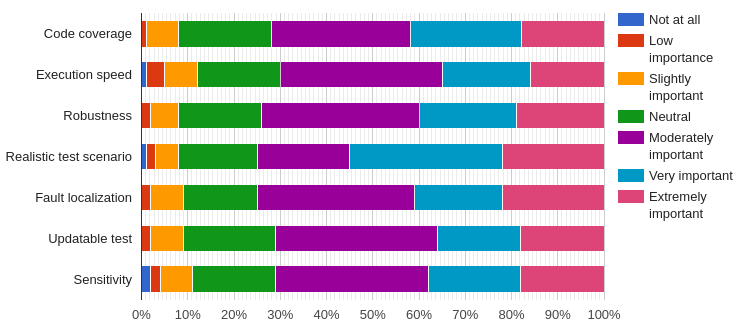
\includegraphics[width=14.7cm]{images/optimize-org.png}
        \caption{Original study~\cite{daka2014survey} unit test optimizing target percentages amongst developers}
        \label{fig:org-optimize}
      \end{center}
    \end{figure}

Regarding JUnit low-level testing, participants in this study had varying importance in studied aspects. Full answers are
displayed in table \ref{tab:changes-pt2} with \textbf{Q3:} \textit{How important are the following aspects for you when you write new low-level tests?}
Participants {\colorbox{lightgray}A} and {\colorbox{lime}B} answered
the most alike, whereas participant {\colorbox{orange}C} had slightly different optimizing profile. \textit{Code coverage}
was a neutral optimizing target for all participants. Additional question original to this study was the \textit{capturing of behavior}
as optimizing target. Participants {\colorbox{lightgray}A} and {\colorbox{lime}B} found it neutral and slightly important,
but participant {\colorbox{orange}C} had it as a very important optimizing target. Another interesting target was \textit{execution speed},
where participants {\colorbox{lightgray}A} and {\colorbox{lime}B} had it at least moderately important, but participant {\colorbox{orange}C}
answered it as low importance optimizing target. \textit{How realistic the test scenario is} was very important to optimize for
participant {\colorbox{orange}C}. This was also the most important target amonst original study survey participants.
For participants {\colorbox{lightgray}A} and {\colorbox{lime}B}, \textit{realistic test scenario} was only slightly important.
These kind of variations in optimizing targets are quite natural when studying this low participant count. The original study
figure \ref{fig:org-optimize} displays how all the targets are quite close to each other with larger sampling.

    \begin{table}[H]
        \resizebox{\textwidth}{!}{%
            \begin{tabular}{p{13.0cm}*{7}{p{2cm}}}
            \topline
            \textbf{Question} & \textbf{Answer options} &  &  &  &   &  & \\ \hline
            \textbf{Q3: How important are the following aspects for you when you write new low-level tests?} & Not at all & Low \newline importance & Slightly important & Neutral & Moderately important & Very \newline important & Extremely important \\
            & \\
            1. Code coverage & 0 & 0 & 0 & {\colorbox{lightgray}A}{\colorbox{lime}B}{\colorbox{orange}C} & 0 & 0 & 0 \\
            2. Capturing all behavior of unit/feature with tests or assertions & 0 & 0 & {\colorbox{lime}B} & {\colorbox{lightgray}A} & 0 & {\colorbox{orange}C} & 0 \\
            3. Execution speed & 0 & {\colorbox{orange}C} & 0 & 0 & {\colorbox{lime}B} & {\colorbox{lightgray}A} & 0 \\
            4. Robustness against code changes (i.e., test does not break easily) & 0 & 0 & 0 & 0 & {\colorbox{lightgray}A}{\colorbox{lime}B}{\colorbox{orange}C} & 0 & 0 \\
            5. How realistic the test scenario is & 0 & 0 & {\colorbox{lightgray}A}{\colorbox{lime}B} & 0 & 0 & {\colorbox{orange}C} & 0 \\
            6. How easily faults can be localised/debugged if the test fails & 0 & 0 & {\colorbox{lime}B} & 0 & {\colorbox{lightgray}A}{\colorbox{orange}C} & 0 & 0 \\
            7. How easily the test can be updated when the underlying code changes & 0 & {\colorbox{orange}C} & {\colorbox{lightgray}A} & 0 & {\colorbox{lime}B} & 0 & 0 \\
            8. Sensitivity against code changes (i.e., test should detect even small code changes) & 0 & {\colorbox{lightgray}A}{\colorbox{lime}B} & 0 & {\colorbox{orange}C} & 0 & 0 & 0 \\
            & \\ \hline
            \textbf{Q3': Compared to JUnit, How important are the following aspects for you when you write new low-level tests?} & A lot less important & Less important & Slightly less important & As important as before & Slightly more important & More important & A lot more important \\
            & \\
            1. Code coverage & 0 & 0 & 0 & {\colorbox{lightgray}A} & 0 & 0 & 0 \\
            2. Capturing all behavior of unit/feature with tests or assertions & 0 & 0 & 0 & 0 & {\colorbox{lightgray}A} & 0 & 0 \\
            3. Execution speed & 0 & 0 & 0 & {\colorbox{lightgray}A} & 0 & 0 & 0 \\
            4. Robustness against code changes (i.e., test does not break easily) & 0 & 0 & 0 & {\colorbox{lightgray}A} & 0 & 0 & 0 \\
            5. How realistic the test scenario is	& 0 & 0 & 0 & {\colorbox{lightgray}A} & 0 & 0 & 0 \\
            6. How easily faults can be localised/debugged if the test fails & 0 & 0 & 0 & 0 & {\colorbox{lightgray}A} & 0 & 0 \\
            7. How easily the test can be updated when the underlying code changes & 0 & 0 & 0 & {\colorbox{lightgray}A} & 0 & 0 & 0 \\
            8. Sensitivity against code changes (i.e., test should detect even small code changes) & 0 & 0 & 0 & {\colorbox{lightgray}A} & 0 & 0 & 0 \\
            & \\ \topline

            \end{tabular}}
            \caption {Optimizing targets in low-level tests and changes in them} \label{tab:changes-pt2}
    \end{table}

The changes in low-level testing optimizing targets were studied with \textbf{Q3':}
\textit{Compared to JUnit, how important are the following aspects for you when you write new low-level tests?}
Participant {\colorbox{lightgray}A} compared the changes from JUnit to \textbf{\textit{Spectrum}} and find most of the targets as important as before.
\textit{Capturing behavior} of tested subject in tests was slightly more important than before. Also \textit{fault localization} was
slightly more important target than before. These two targets and their higher importance seem natural for a \textbf{xSpec family}
testing framework, as it aims to promote more granular and more natural language description information holding test cases than JUnit.

\textbf{TO BE CONTINUED}
\clearpage
\subsubsection{Test understandability and informativeness }
The difficulty of developers \textbf{understanding} unit tests was studied by Li et al.~\cite{li2016automatically}. Over 60\% of survey
participants found it at least moderately difficulty. Figure \ref{fig:org-understandability} illustrates the total survey
answer regarding unit test understandability. This question was chosen to be replicated in this study to see, if the research
hypothesis of developers finding it easier to understand test cases with BDD testing frameworks will hold true.

    \begin{figure}[ht]
      \begin{center}
        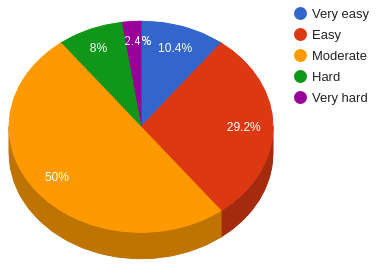
\includegraphics[width=7.7cm]{images/org-understandability.png}
        \caption{Original study~\cite{li2016automatically} unit test understandability}
        \label{fig:org-understandability}
      \end{center}
    \end{figure}

Table \ref{tab:changes-pt3} summarizes this study participant answers. First \textbf{Q4} studied how difficult understanding
of low-level tests with JUnit was. The results mirrored quite well the original study findings, as participants {\colorbox{lime}B} and {\colorbox{orange}C}
find the understandability to be moderately diffucult and participant {\colorbox{lightgray}A} found it hard to understand a low-level test.


    \begin{table}[H]
        \resizebox{\textwidth}{!}{%
            \begin{tabular}{p{13.0cm}*{7}{p{2cm}}}
            \topline
            \textbf{Question} & \textbf{Answer options} &  &  &  &   &  & \\ \hline
            & Very easy & Easy & Moderate & Hard & Very hard & & \\
            & \\
            \textbf{Q4: How difficult is it for you to understand a low-level test?} & 0 & 0 & {\colorbox{lime}B}{\colorbox{orange}C} & {\colorbox{lightgray}A} & 0 \\
            & \\ \hline
            & A lot less difficult & Less difficult & Slightly less difficult & As difficult as before & Slightly more difficult & More difficult & A lot more difficult \\
            & \\
            \textbf{Q4': Compared to JUnit, how difficult is it for you to understand a low-level test?} & 0 & {\colorbox{lightgray}A} & 0 & 0 & 0 & 0 & 0 \\
            & \\ \topline
            \end{tabular}}
            \caption {Understandability of low-level tests and changes in it} \label{tab:changes-pt3}
    \end{table}

The changes in low-level test understandability were studied with \textbf{Q4':} \textit{Compared to JUnit, how difficult is it
for you to understand a low-level test?} Participant {\colorbox{lightgray}A} found it less difficult to understand a low-level
test after the introduction of \textbf{\textit{Spectrum}}.

Table \ref{tab:changes-pt4} displays questions \textbf{Q5 \& Q5'} and their results. Q5 was chosen to see first
how easily the JUnit test methods can be \textbf{structured} and \textbf{understood} to hold different parts of the test. JUnit testing literature states that
the structure should be done with \textit{Arrange-Act-Assert}~\cite{langr2015pragmatic}, but it is not enforced and thus can lead to poorly structured
tests which are hard to understand~\cite{kapelonis2016java}. Q5 studies if this does hold true.

All the participants had different parts of test
structure with ranging difficulties in structuring and understanding. Participant {\colorbox{lightgray}A} could be categorized to hold almost all
parts of structuring the test somewhat difficult, with the exception of finding it easy to structure information to context of tests.
Reading tests and understanding their structure was found at least from slightly hard to hard.
Participant {\colorbox{lime}B} find writing information to assertions of test easy, but otherwise structuring the test
was found from moderately difficult to slightly hard. Reading the test structure parts for information was equivalent
to writing and structuring of tests. Participant {\colorbox{orange}C} found it somewhat difficult to produce information
to tests, but reading the test structure was found to be slightly easy. These ranging results are not too surprising,
as JUnit does not promote a certain structure for tests. It seems to result in hard to produce stucture that is not
too easy to understand.

    \begin{table}[H]
        \resizebox{\textwidth}{!}{%
            \begin{tabular}{p{13.0cm}*{7}{p{2cm}}}
            \topline
            \textbf{Question} & \textbf{Answer options} &  &  &  &   &  & \\ \hline
            \textbf{Q5: In low-level testing, how difficult is it for you to} & Very easy & Easy & Slightly easy & Moderate & Slightly hard & Hard & Very hard \\
            & & & & & & \\
            1. Structure and write information to context of test? & 0 & {\colorbox{lightgray}A} & 0 & 0 & {\colorbox{lime}B}{\colorbox{orange}C} & 0 & 0 \\
            2. Structure and write information to stimulus of test? & 0 & 0 & 0 & {\colorbox{lightgray}A}{\colorbox{lime}B}{\colorbox{orange}C} & 0 & 0 & 0 \\
            3. Structure and write information to assertions of test? & 0 & {\colorbox{lime}B} & {\colorbox{orange}C} & 0 & {\colorbox{lightgray}A} & 0 & 0 \\
            4. Read test case structure for information about context of test? & 0 & 0 & {\colorbox{orange}C} & 0 & {\colorbox{lime}B} & {\colorbox{lightgray}A} & 0 \\
            5. Read test case structure for information about stimulus of test? & 0 & 0 & {\colorbox{orange}C} & {\colorbox{lime}B} & {\colorbox{lightgray}A} & 0 & 0 \\
            6. Read test case structure for information about assertions of test? & 0 & {\colorbox{lime}B} & {\colorbox{orange}C} & 0 & 0 & {\colorbox{lightgray}A} & 0 \\
            & \\ \hline
            \textbf{Q5': Compared to JUnit in low-level testing, how difficult is it for you to} & A lot less difficult & Less difficult & Slightly less difficult & As difficult as before & Slightly more difficult & More difficult & A lot more difficult \\
            & & & & & & \\
            1. Structure and write information to context of test? & {\colorbox{lightgray}A} & 0 & 0 & 0 & 0 & 0 & 0 \\
            2. Structure and write information to stimulus of test? & 0 & {\colorbox{lightgray}A} & 0 & 0 & 0 & 0 & 0 \\
            3. Structure and write information to assertions of test? & 0 & 0 & {\colorbox{lightgray}A} & 0 & 0 & 0 & 0 \\
            4. Read test case structure for information about context of test? & 0 & 0 & {\colorbox{lightgray}A} & 0 & 0 & 0 & 0 \\
            5. Read test case structure for information about stimulus of test? & 0 & {\colorbox{lightgray}A} & 0 & 0 & 0 & 0 & 0 \\
            6. Read test case structure for information about assertions of test? & 0 & 0 & {\colorbox{lightgray}A} & 0 & 0 & 0 & 0 \\
            & \\ \topline
            \end{tabular}}
            \caption {Low-level test structure informativiness and changes in it} \label{tab:changes-pt4}
    \end{table}

Q5' displays the changes in structuring and reading of tests for information. Participant {\colorbox{lightgray}A} found \textbf{\textit{Spectrum}}
on all occasions easier to structure information to tests and also to read it from tests. Structuring information to
tests could be categorized as quite much easier. Reading the tests for information was found somewhat easier than with JUnit.
\clearpage

Table \ref{tab:changes-pt5} displays questions \textbf{Q6 \& Q6'} with results. First Q6 studies how \textbf{informative} participants
found JUnit test output. Participant {\colorbox{lightgray}A} find the output hardly informative, whereas participants {\colorbox{lime}B}
and {\colorbox{orange}C} found the output ranging from somewhat informative to moderately informative. These results are
not too suprising, as normal JUnit test method naming do not tend hold that much words. Section \ref{subsub:low-level-metrics} displays
that the average word count in test methods in projects were ranging from approximately 5 to 6. This amount of words can't
hold naturally too much information in total.

    \begin{table}[H]
        \resizebox{\textwidth}{!}{%
            \begin{tabular}{p{13.0cm}*{7}{p{2cm}}}
            \topline
            \textbf{Question} & \textbf{Answer options} &  &  &  &   &  & \\ \hline
            & Not at all & Hardly informative & Slightly informative & Somewhat informative & Moderately informative & Very informative & Extremely informative \\
            & \\
            \textbf{Q6: How informative you usually find the test output?} & 0 & {\colorbox{lightgray}A} & 0 & {\colorbox{orange}C} & {\colorbox{lime}B} & 0 & 0 \\
            & \\ \hline
            & A lot less informative & Less informative & Slightly less informative & As informative as before & Slightly more informative & More informative & A lot more informative \\
            & \\
            \textbf{Q6': Compared to JUnit, how informative you usually find the test output?} & 0 & 0 & 0 & 0 & {\colorbox{lightgray}A} & 0 & 0 \\
            & \\ \topline

            \end{tabular}}
            \caption {Low-level test output informativeness and changes in it} \label{tab:changes-pt5}
    \end{table}

Q6' studies the change of test output informativeness after the introduction of new BDD testing framework. Participant {\colorbox{lightgray}A}
found a slight increase in informativeness of output.

\clearpage
\subsubsection{Test refactoring techniques}

Table \ref{tab:changes-pt6} displays the usage of different \textbf{repetition reducing} techniques. First \textbf{Q7:}
\textit{How much are the following repetition reducing techniques used in your low-level testing?} studies how much a
set of common refactoring techniques stated in unit testing literature ~\cite{artofunit2013} are used in projects.

Most common used refactoring techniques amongst survey participants were \textit{extract method} and lifecycle hook \textit{before -each}.
These two techniques were in use frequently or very frequently within participant testing. Lifecycle hook \textit{before -class} was also
in use at least occasionally. Automatic test generation through DDT was found very rarely or rarely used with participants {\colorbox{lightgray}A}
and {\colorbox{lime}B}. Section \ref{subsub:low-level-metrics} shows that in project A it was not used at all, where data-driven test method ratio to standard
low level test methods was 0. Participant {\colorbox{orange}C} answered to use occasionally DDT and the test code analysis
data in section \ref{subsub:low-level-metrics} supported this. Common test initializer class inheritance was a practice
very rarely or rarely used amongst all participants. During interview, participant {\colorbox{lightgray}A} even stated test class inheritance
to be \textit{"a practice to avoid, it's devil's work"}.

    \begin{table}[H]
        \resizebox{\textwidth}{!}{%
            \begin{tabular}{p{13.0cm}*{7}{p{2cm}}}
            \topline
            \textbf{Question} & \textbf{Answer options} &  &  &  &   &  & \\ \hline
            \textbf{Q7: How much are the following repetition reducing techniques used in your low-level testing?} & Never & Very rarely & Rarely & Occasionally & Frequently & Very \newline frequently & Always \\
            & & & & & & \\
            1. Extract method (custom helper methods) & 0 & 0 & 0 & 0 & {\colorbox{lightgray}A}{\colorbox{lime}B} & {\colorbox{orange}C} & 0 \\
            2. Lifecycle hooks Before/After (class) & 0 & 0 & 0 & {\colorbox{orange}C} & {\colorbox{lightgray}A}{\colorbox{lime}B} & 0 & 0 \\
            3. Lifecycle hooks Before/After (each) & 0 & 0 & 0 & 0 & {\colorbox{lightgray}A}{\colorbox{lime}B} & {\colorbox{orange}C} & 0 \\
            4. Automatic test generation via test method parametrization & 0 & {\colorbox{lightgray}A} & {\colorbox{lime}B} & {\colorbox{orange}C} & 0 & 0 & 0 \\
            5. Common test initializer class inheritance & 0 & {\colorbox{lightgray}A}{\colorbox{orange}C} & {\colorbox{lime}B} & 0 & 0 & 0 & 0 \\
            & \\ \hline

            \textbf{Q7': Compared to JUnit, how much are the following repetition reducing techniques used in your low-level testing?} & A lot less & Less & Slightly less & The same amount & Slightly more & More & A lot more \\
            & & & & & & \\
            1. Extract method (custom helper methods) & 0 & 0 & 0 & {\colorbox{lightgray}A} & 0 & 0 & 0 \\
            2. Lifecycle hooks Before/After (class/all) & 0 & 0 & 0 & {\colorbox{lightgray}A} & 0 & 0 & 0 \\
            3. Lifecycle hooks Before/After (each) & 0 & 0 & 0 & 0 & 0 & {\colorbox{lightgray}A} & 0 \\
            4. Automatic test generation via test method parametrization & 0 & 0 & 0 & {\colorbox{lightgray}A} & 0 & 0 & 0 \\
            5. Common test initializer class inheritance & 0 & 0 & 0 & {\colorbox{lightgray}A} & 0 & 0 & 0 \\
            & \\ \topline

            \end{tabular}}
            \caption {Used repetition reducing techniques for low-level testing and changes in their use} \label{tab:changes-pt6}
    \end{table}

\textbf{Q7':} \textit{Compared to JUnit, how much are the following repetition reducing techniques used in your low-level testing?}
studies how techniques are used differently with the new BDD testing framework to reduce repetition. Participant {\colorbox{lightgray}A}
said to use techniques the same amount as before, with the exception of lifecycle hook \textit{before -each} being used more.
In the feedback interview, participant {\colorbox{lightgray}A} stated that there was some confusion when to use \textit{before -all}
lifecycle hook and therefore hook \textit{before -each} was mainly used.

\textbf{TO BE CONTINUED}
\clearpage
\subsubsection{Test commenting practices}
    \begin{figure}[ht]%
        \centering
        \subfloat[Comment adding ]{{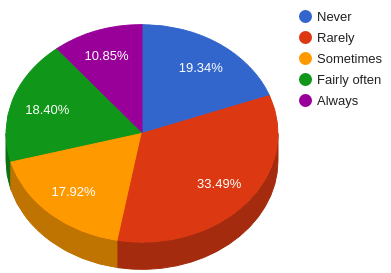
\includegraphics[width=6.75cm]{images/org-add-document.png} }}%
        \qquad
        \subfloat[Comment updating]{{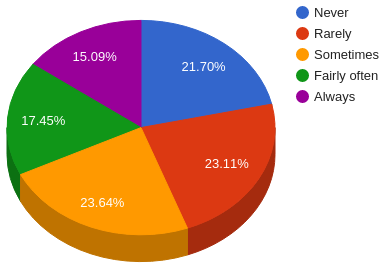
\includegraphics[width=6.75cm]{images/org-update-document.png} }}%
        \caption{Original study~\cite{li2016automatically} unit testing commenting practices}%
        \label{fig:org-commenting}%
    \end{figure}

Test commenting and comment updating was found to be a practice rarely done by most of the developers~\cite{li2016automatically}.
Figure \ref{fig:org-commenting} shows the original study results regarding test commenting practices. Participants in this
study seem to divide with commenting practices. Table \ref{tab:changes-pt7} displays the participant JUnit commenting practice results with
\textbf{Q8} and \textbf{Q9}. Project A and its participants {\colorbox{lightgray}A} and {\colorbox{lime}B}
answer fairly often to add and update comments in low-level test cases. Participant {\colorbox{orange}C} rarely practices
test commenting or updating. Test data analysis in \ref{subsub:low-level-metrics} correlates with participant answers, as
project A had quite much commenting in test methods and project B very little.

    \begin{table}[H]
        \resizebox{\textwidth}{!}{%
            \begin{tabular}{p{13.0cm}*{7}{p{2cm}}}
            \topline
            \textbf{Question} & \textbf{Answer options} &  &  &  &   &  & \\ \hline
            & Never & Rarely & Sometimes & Fairly often & Always & & \\
            & \\
            \textbf{Q8: How often do you add/write documentation comments to low-level test cases?} & 0 & {\colorbox{orange}C} & 0 & {\colorbox{lightgray}A}{\colorbox{lime}B} & 0 \\
            & \\ \hline
            & A lot less & Less & Slightly less & The same amount & Slightly more & More & A lot more \\
            & \\
            \textbf{Q8': Compared to JUnit, how often do you add/write documentation comments to low-level test cases?} & 0 & 0 & 0 & 0 & 0 & {\colorbox{lightgray}A} & 0 \\
            & \\ \hline

            & Never & Rarely & Sometimes & Fairly often & Always & & \\
            & \\
            \textbf{Q9: When you make changes to low-level tests, how often do you comment the changes (or update existing comments)?} & 0 & {\colorbox{orange}C} & 0 & {\colorbox{lightgray}A}{\colorbox{lime}B} & 0 \\
            & \\ \hline
            & A lot less & Less & Slightly less & The same amount & Slightly more & More & A lot more \\
            & \\
            \textbf{Q9': Compared to JUnit when you make changes to low-level tests, how often do you comment the changes (or update existing comments)?} & 0 & 0 & 0 & 0 & {\colorbox{lightgray}A} & 0 & 0 \\
            & \\ \topline

            \end{tabular}}
            \caption {Documentation practices in low-level testing and changes in them} \label{tab:changes-pt7}
    \end{table}

Questions \textbf{Q8'} and \textbf{Q9'} in table \ref{tab:changes-pt7} study the changes in commenting with new BDD testing framework.
Participant {\colorbox{lightgray}A} answers to add more comments with \textbf{\textit{Spectrum}} to low-level test cases
than before and also to update the comments slightly more.
%TODO kato taaaaa kaymaan toteen
Here the test code analysis data in section \ref{subsub:low-level-metrics} doesn't support this directly, as pure comments
in test methods have decreased. But overall
the test contains more textual description in use with code example group and code example descriptions, which can be seen
as increased test method name word count.

\textbf{TO BE CONTINUED}
\clearpage
\subsubsection{Unit testing practices}
Pure unit testing practices were also studied with the participant surveys. First the \textbf{granularity} of unit tests were
studied with questions \textbf{Q10} and \textbf{Q10'} displayed in table \ref{tab:changes-pt8}. Participants {\colorbox{lightgray}A} and {\colorbox{lime}B} answered
to write approximately two to three tests methods per class method that contain few assertions inside them each. Participant
{\colorbox{orange}C} answered to produce more granular test cases, where there exists four to five test methods per class method.
Also the assertion count was stated to be higher, 4-5 assertions per test method. Test data analysis in section \ref{subsub:unit-level-metrics}
seems to support quite well all these participant answers, although the assertion count per test method calculated in section \ref{subsub:low-level-metrics}
for project B was slightly lower than the answered four to five assertions per test method.

    \begin{table}[H]
        \resizebox{\textwidth}{!}{%
            \begin{tabular}{p{13.0cm}*{7}{p{2cm}}}
            \topline
            \textbf{Question} & \textbf{Answer options} &  &  &  &   &  & \\ \hline
            \textbf{Q10: In unit testing, how many} & 0 & 1 & 2-3 & 4-5 & 6-7 &  8-9 & 10 or more \\
            & \\
            1. Test methods do you usually write per class method? & 0 & 0 & {\colorbox{lightgray}A}{\colorbox{lime}B} & {\colorbox{orange}C} & 0 & 0 & 0 \\
            2. Assertions do you usually write per test method? & 0 & 0 & {\colorbox{lightgray}A}{\colorbox{lime}B} & {\colorbox{orange}C} & 0 & 0 & 0 \\
            & \\ \hline
            \textbf{Q10': Compared to JUnit in unit testing} & A lot less & Less & Slightly less & The same amount & Slightly more & More & A lot more \\
            & \\
            1. Do you write more or less test methods per class method? & 0 & 0 & 0 & 0 & 0 & {\colorbox{lightgray}A} & 0 \\
            2. Do you write more or less assertions per test method? & 0 & {\colorbox{lightgray}A} & 0 & 0 & 0 & 0 & 0 \\
            & \\ \topline

             \end{tabular}}
             \caption {Unit testing practices and changes in them} \label{tab:changes-pt8}
     \end{table}

Changes in unit testing granularity after introduction of BDD testing framework were studied with Q10'. Participant {\colorbox{lightgray}A}
answered that with \textbf{\textit{Spectrum}} he wrote more test methods per class method with less assertion inside individual
test methods.

\clearpage

In related research, survey participant developers found unit test \textbf{isolation} to be a demanding practice~\cite{daka2014survey}.
Therefore questions \textbf{Q11, Q11', Q12} and \textbf{Q12'} displayed in table \ref{tab:changes-pt9} are aimed to learn more about isolation in unit testing.
First survey question Q11 asks what mocking library is normally used in JUnit unit test isolation. After that,
\textbf{Q12} studies wich aspects of isolating are find hard.

Usually unit test isolation is done with \textit{Mockito} by all participants. Participant {\colorbox{orange}C} is the only
one that found all aspects of unit test isolation to be easy or slightly easy. Participant {\colorbox{lightgray}A} found isolation
usually slightly easy with \textit{verifying} of mock object actions being moderate in difficulty. Participant {\colorbox{lime}B}
found most of isolation easy, but \textit{stubbing} was considered slightly hard. Altogether, isolation activities in JUnit unit testing
wasn't found too demanding by any of the participants.

    \begin{table}[H]
        \resizebox{\textwidth}{!}{%
            \begin{tabular}{p{13.0cm}*{7}{p{2cm}}}
            \topline
            \textbf{Question} & \textbf{Answer options} &  &  &  &   &  & \\ \hline
            & Mockito & jMock & Powermock & Easymock & Other & & \\
             \\
            \textbf{Q11: In unit testing, what mocking library do you normally use?} & {\colorbox{lightgray}A}{\colorbox{lime}B}{\colorbox{orange}C} & 0 & 0 & 0 & 0 \\
            & \\ \hline
            & \textit Mockito & jMock & Powermock & Easymock & Spock's internal mocking & Other & \\
            & \\
            \textbf{Q11': In unit testing with \textit{Spectrum/Spock}, what mocking library do you normally use?} & {\colorbox{lightgray}A} & 0 & 0 & 0 & 0 & 0 \\
            & \\ \hline

            \textbf{Q12: In unit testing, how difficult you find it to} & Very easy & Easy & Slightly easy & Moderate & Slightly hard & Hard & Very hard \\
            & \\
            1. Mock objects? & 0 & {\colorbox{lime}B}{\colorbox{orange}C} & {\colorbox{lightgray}A} & 0 & 0 & 0 & 0 \\
            2. Stub method calls? & 0 & 0 & {\colorbox{lightgray}A}{\colorbox{orange}C} & 0 & {\colorbox{lime}B} & 0 & 0 \\
            3. Verify mock object actions? & 0 & {\colorbox{lime}B}{\colorbox{orange}C} & 0 & {\colorbox{lightgray}A} & 0 & 0 & 0 \\
            & \\ \hline
            \textbf{Q12': Compared to JUnit in unit testing, how difficult you find it to} & A lot easier & Easier & Slightly easier & As difficult as before & Slightly harder & Harder & A lot harder \\
            & \\
            1. Mock objects? & 0 & 0 & 0 & 0 & {\colorbox{lightgray}A} & 0 & 0 \\
            2. Stub method calls? & 0 & 0 & 0 & 0 & {\colorbox{lightgray}A} & 0 & 0 \\
            3. Verify mock object actions? & 0 & 0 & 0 & 0 & {\colorbox{lightgray}A} & 0 & 0 \\
            & \\ \topline

            \end{tabular}}
            \caption {Unit testing practices and changes in them} \label{tab:changes-pt9}
    \end{table}

After the introduction of \textbf{\textit{Spectrum}} in project A, the mocking library stayed intact as Spectrum
is a Java-based custom runner for JUnit. Although the mocking library was the same, participant {\colorbox{lightgray}A}
found all aspects on unit test isolation slightly harder than before. This was further analyzed in interview with participant,
where he states that the usage of \textit{Mockito}-functions inside \textbf{lifecycle hooks} and \textbf{block lambdas} was not
as straightforward as with JUnit tests.
\clearpage

Questions \textbf{Q13} and \textbf{Q13'} were aimed to study when are unit tests add for code with JUnit and the new
BDD testing framework. The main idea was to see, does the introduction of BDD testing framework by itself promote test firsts -principle without
additional changes in testing. For participant {\colorbox{lightgray}A} there was no change, as the unit tests were added
after the implementation with both JUnit and \textbf{\textit{Spectrum}}}.

    \begin{table}[H]
        \resizebox{\textwidth}{!}{%
            \begin{tabular}{p{13.0cm}*{7}{p{2cm}}}
            \topline
            \textbf{Question} & \textbf{Answer options} &  &  &  &   &  & \\ \hline
            & Before implementation & During implementation & After implementation & \\
            & \\
            \textbf{Q13: When do you add automated unit tests for developed code with \textit{JUnit}?} & 0 & {\colorbox{lime}B}{\colorbox{orange}C} & {\colorbox{lightgray}A} \\
            & \\ \hline
            & Before implementation & During implementation & After implementation & \\
            & \\
            \textbf{Q13': When do you add automated unit tests for developed code with \textit{Spectrum/Spock}?} & 0 & 0 & {\colorbox{lightgray}A} \\
            & \\ \topline

            \end{tabular}}
            \caption {Unit testing practices and changes in them} \label{tab:junit-pt1}
    \end{table}

\subsubsection{Change summary}

\clearpage


\subsection{Developer perception towards automated low-level testing}
This section answer the
\textbf{RQ2: }\textit{How does behavior driven testing frameworks change developer perception of working with automated low-level
testing compared to JUnit framework?} First, developer perception of automated low-level testing and changes in it are
analyzed with survey and interviews. Second, developer loyalty towards low-level automated testing and specific testing
frameworks are studied with \textbf{NPS} survey questions and further studied with interviews.

\subsubsection{Developer perception of low-level testing}
    \begin{figure}[ht]
      \begin{center}
        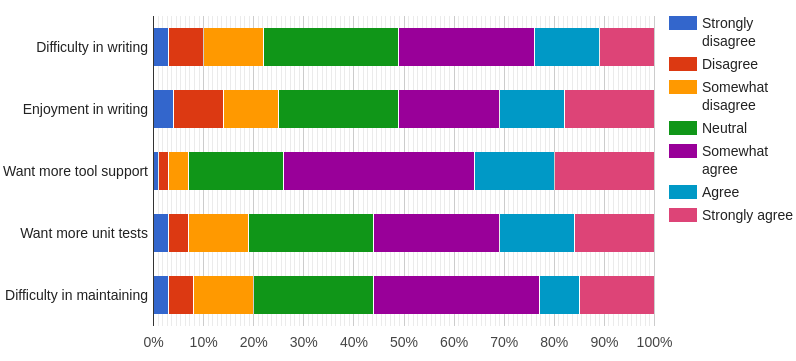
\includegraphics[width=14.7cm]{images/perception-org.png}
        \caption{Original study~\cite{daka2014survey} developer perception of unit testing}
        \label{fig:TDD}
      \end{center}
    \end{figure}

    \begin{figure}[ht]%
        \centering
        \subfloat[Unit tests help in producing higher quality code~\cite{williams2009effectiveness}]{{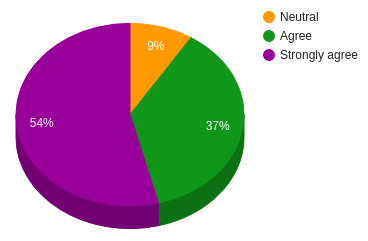
\includegraphics[width=6.75cm]{images/org-quality.png} }}%
        \qquad
        \subfloat[Maintaining unit tests is important for the quality of the system~\cite{li2016automatically}]{{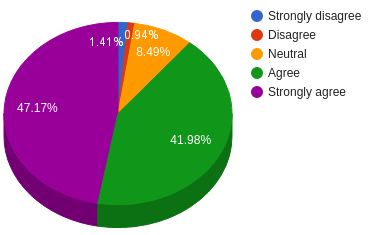
\includegraphics[width=6.75cm]{images/org-maintaining.png} }}%
        \caption{Developer perception of unit testing in original studies}%
        \label{fig:example}%
    \end{figure}

    \begin{table}[H]
        \resizebox{\textwidth}{!}{%
            \begin{tabular}{p{13.0cm}*{7}{p{2cm}}}
            \topline
            \textbf{Question} & \textbf{Answer options} &  &  &  &   &  & \\ \hline

            \textbf{Q14: Please indicate your level of agreement with the following statements} & Strongly disagree & Disagree & Somewhat disagree & Neither agree nor disagree & Somewhat agree & Agree & Strongly agree \\
            & \\
            1. Writing low-level tests is difficult & 0 & 0 & {\colorbox{orange}C} & 0 & {\colorbox{lightgray}A}{\colorbox{lime}B} & 0 & 0 \\
            2. I enjoy writing low-level tests & 0 & {\colorbox{lime}B} & 0 & {\colorbox{lightgray}A} & 0 & {\colorbox{orange}C} & 0 \\
            3. I would like to have more tool support when writing low-level tests & 0 & 0 & {\colorbox{lime}B} & {\colorbox{lightgray}A} & {\colorbox{orange}C} & 0 & 0 \\
            4. I would like to have more low-level tests & 0 & 0 & 0 & {\colorbox{lightgray}A}{\colorbox{lime}B}{\colorbox{orange}C} & 0 & 0 & 0 \\
            5. Maintaining low-level tests is difficult & 0 & 0 & {\colorbox{orange}C} & 0 & {\colorbox{lime}B} & {\colorbox{lightgray}A} & 0 \\
            6. I think my low-level tests will help other developers to understand the implemented unit/feature better & 0 & 0 & {\colorbox{lime}B} & 0 & {\colorbox{lightgray}A} & {\colorbox{orange}C} & 0 \\
            7. Low-level automated testing helps me find defects in the code before other quality assurance phases & 0 & 0 & 0 & 0 & {\colorbox{lime}B} & {\colorbox{orange}C} & {\colorbox{lightgray}A} \\
            8. JUnit promotes me to write high quality test code & 0 & 0 & {\colorbox{lightgray}A}{\colorbox{orange}C} & {\colorbox{lime}B} & 0 & 0 & 0 \\
            & \\ \hline

            \textbf{Q15a: Please indicate your level of agreement with the following statements} & Strongly disagree & Disagree & Neutral & Agree & Strongly agree & \\
            & \\
            1. Overall, low-level tests help me produce higher quality code & 0 & 0 & 0 & {\colorbox{lime}B} & {\colorbox{lightgray}A}{\colorbox{orange}C} \\
            2. Maintaining good low-level test cases and their documentations is important to the quality of a system & 0 & 0 & 0 & {\colorbox{lightgray}A}{\colorbox{lime}B} & {\colorbox{orange}C} \\
            & \\ \topline

            \end{tabular}}
            \caption {Developer perception of low-level testing with JUnit} \label{tab:junit-pt2}
    \end{table}

    \begin{table}[H]
        \resizebox{\textwidth}{!}{%
            \begin{tabular}{p{13.0cm}*{7}{p{2cm}}}
            \topline
            \textbf{Question} & \textbf{Answer options} &  &  &  &   &  & \\ \hline
            \textbf{Q14'\&Q15a': Please indicate your level of agreement with the following statements} & Strongly disagree & Disagree & Somewhat disagree & Neither agree nor disagree & Somewhat agree & Agree & Strongly agree \\
            & \\
            1. Writing low-level tests with \textit{Spectrum/Spock} is more difficult than with JUnit & 0 & 0 & 0 & 0 & {\colorbox{lightgray}A} & 0 & 0 \\
            2. I enjoy writing low-level tests with \textit{Spectrum/Spock} more than I do with JUnit & 0 & 0 & 0 & 0 & {\colorbox{lightgray}A} & 0 & 0 \\
            3. I would like to have more tool support for \textit{Spectrum/Spock} when writing low-level tests & 0 & 0 & 0 & 0 & 0 & 0 & {\colorbox{lightgray}A} \\
            4. I would like to have more low-level tests for \textit{Spectrum/Spock} & 0 & 0 & 0 & 0 & {\colorbox{lightgray}A} & 0 & 0 \\
            5. Maintaining low-level tests with \textit{Spectrum/Spock} is more difficult than with JUnit & 0 & 0 & 0 & 0 & {\colorbox{lightgray}A} & 0 & 0 \\
            6. I think my low-level tests with \textit{Spectrum/Spock} will help other developers to understand the implemented unit/feature better than earlier tests with JUnit & 0 & 0 & 0 & 0 & 0 & {\colorbox{lightgray}A} & 0 \\
            7. Low-level automated testing with \textit{Spectrum/Spock} helps me find defects in the code before other quality assurance phases better than earlier tests with JUnit & 0 & 0 &  {\colorbox{lightgray}A} & 0 & 0 & 0 & 0 \\
            8. \textit{Spectrum/Spock} promotes me to write higher quality test code than with JUnit & 0 & 0 & 0 & 0 & 0 &  {\colorbox{lightgray}A} & 0 \\ \hline
            & \\
            9. Overall, low-level tests with \textit{Spectrum/Spock} help me produce higher quality code than with JUnit & 0 & 0 &  {\colorbox{lightgray}A} & 0 & 0 & 0 & 0 \\
            10. Maintaining good low-level test cases and their documentation with \textit{Spectrum/Spock} is more important for system quality than maintaining JUnit test cases & 0 & 0 & 0 & 0 & {\colorbox{lightgray}A} & 0 & 0 \\
            & \\ \topline

            \end{tabular}}
            \caption {Developer perception changes in low-level testing with \textit{Spectrum/Spock}} \label{tab:junit-pt2}
    \end{table}
    \vspace{20px}


    \begin{table}[H]
        \resizebox{\textwidth}{!}{%
            \begin{tabular}{p{15.0cm}*{3}{p{2.0cm}}}
            \topline
            \textbf{Question} & \textbf{Answer options} &  &  \\ \hline

            \textbf{Q15b: I would say that I write more} & Yes & Uncertain & No \\
            & \\
            1. Understandable low-level tests with \textit{Spectrum/Spock} than with JUnit? & {\colorbox{lightgray}A} & 0 & 0 \\
            2. Maintainable low-level tests with \textit{Spectrum/Spock} than with JUnit? & {\colorbox{lightgray}A} & 0 & 0  \\
            & \\ \topline

            \end{tabular}}
            \caption {Developer perception towards \textit{Spectrum/Spock}} \label{tab:spock-spectrum-pt3}

    \end{table}


\subsubsection{Developer loyalty towards low-level testing}

    \begin{table}[H]
        \resizebox{\textwidth}{!}{%
            \begin{tabular}{p{17.0cm}*{11}{p{1cm}}}
            \topline
            \textbf{Question} & \multicolumn{3}{l}{\textbf{Answer options}} & \\
            & \\ \hline
            & \multicolumn{4}{l}{\textit{Not at all likely}} & & & & \multicolumn{4}{r}{\textit{Extremely likely}} \\
            \textbf{Q16: How likely are you to} & 0 & 1 & 2 & 3 & 4 & 5 & 6 & 7 & 8 & 9 & 10 \\
            & \\
            1. Recommend low-level automated testing for colleague as a software development practice? & 0 & 0 & 0 & 0 & 0 & 0 & 0 & 0 & {\colorbox{lime}B} & 0 & {\colorbox{lightgray}A}{\colorbox{orange}C} \\
            2. Recommend testing framework JUnit for future Spring projects where you take part in existing project? & 0 & 0 & 0 & 0 & 0 & 0 & 0 & {\colorbox{orange}C} & 0 & {\colorbox{lime}B} & {\colorbox{lightgray}A} \\
            3. Take testing framework JUnit in use for future Spring projects where you have technical lead role in a new starting project? & 0 & 0 & 0 & 0 & 0 & 0 & 0 & 0 & {\colorbox{orange}C} & {\colorbox{lime}B} & {\colorbox{lightgray}A} \\
            & \\ \hline
            & \multicolumn{4}{l}{\textit{Not at all likely}} & & & & \multicolumn{4}{r}{\textit{Extremely likely}} \\
            \textbf{Q16': How likely are you to} & 0 & 1 & 2 & 3 & 4 & 5 & 6 & 7 & 8 & 9 & 10 \\
            & \\
            1. Recommend low-level automated testing for colleague as a software development practice? & 0 & 0 & 0 & 0 & 0 & 0 & 0 & 0 & 0 & 0 & {\colorbox{lightgray}A} \\
            2. Recommend testing framework \textit{Spectrum/Spock} for future Spring projects where you take part in existing project? & 0 & 0 & 0 & 0 & 0 & 0 & {\colorbox{lightgray}A} & 0 & 0 & 0 & 0 \\
            3. Take testing framework \textit{Spectrum/Spock} in use for future Spring projects where you have technical lead role in a new starting project? & 0 & 0 & 0 & 0 & 0 & 0 & {\colorbox{lightgray}A} & 0 & 0 & 0 & 0 \\
            & \\ \topline

            \end{tabular}}
            \caption {NPS questions related to JUnit and \textit{Spectrum/Spock}} \label{tab:junit-pt3}

    \end{table}

    \clearpage

\subsubsection{Change summary}

\section{Test code analysis}
Test code analysis was done to answer \textbf{RQ3} with metrics defined in chapter \ref{chapter:methods} section \ref{subsub:test}.
Test code analysis was done with master branches of projects A and B, \textbf{before} and \textbf{after} the introduction of new BDD testing framework, to related
low-level tests and their affected components. First the unit testing level changes are inspected with projects A and B.
After this, the low-level testing metrics and changes in them are demonstrated with both projects.

\subsection{Automated unit testing level}
\label{subsub:unit-level-metrics}
At automated unit testing level, two metrics were used to study the changes in unit testing: average \textbf{count of test methods}
per tested class methods and \textbf{code coverage}. Table \ref{tab:unit-metrics} displays these values before the introduction
of new BDD testing framework and after. In \textbf{COTM} before values are calculated for JUnit unit tests only and after
values only for new unit tests done with the selected BDD testing framework. In \textbf{CC}, before values are for the
whole project at unit level with JUnit. After values are unit testing coverage for JUnit and new BDD testing framework
combined.

{\renewcommand{\arraystretch}{1.3}
\begin{table}[H]
    \resizebox{\textwidth}{!}{%
        \begin{tabular}{p{6.0cm}*{4}{p{3cm}}}

        \headcol \textbf{Metric} & \textbf{Project A} \newline JUnit & \textbf{Project A} \newline Spectrum & \textbf{Project B} \newline JUnit & \textbf{Project B} \newline Spock  \\ \hline

        \rowcol \textit{\textbf{COTM}} & \textbf{1.44} & & \textbf{3.49} & \\
        \rowcol \textit{Sum of tested class methods} & 61 &  & 93 & \\
        \rowcol \textit{Sum of unit test methods} & 88 & & 325 & \\ \hline

        \textit{\textbf{Instruction CC}} & \textbf{25\%} & & \textbf{20\%} & \\
        \textit{Total number of instructions} & 31,425 & & 49,895 & \\
        \textit{\textbf{Branch CC}} & \textbf{24\%} & & \textbf{20\%} & \\
        \textit{Total number of branches} & 724 & & 2,195 & \\ \bottomlinec
        \end{tabular}}
        \caption {Unit level testing metrics in projects and their change} \label{tab:unit-metrics}

\end{table}
}

\textbf{RQ3: }\textit{How does behavior driven testing frameworks change written low-level test cases and test code coverage compared to JUnit framework?}
is first studied with data from unit testing metrics displayed in table \ref{tab:unit-metrics}.

\clearpage
\subsection{Automated unit \& integration testing levels}
\label{subsub:low-level-metrics}
At automated low-level testing level there were 5 inspected metrics: \textbf{code coverage}, average \textbf{count of assertions} per test method,
average \textbf{count of comments} per test method, average \textbf{test method name word count} and ratio of \textbf{data driven test methods} to
all low-level test methods. \textbf{CC} is measured as combined JUnit and new BDD framework coverage. All other metrics
are measured first from existing low-level JUnit tests and after from new BDD testing framework specifications.
Table \ref{tab:low-metrics} dislays the values of these metrics in projects A and B before and after introduction of BDD testing framework.


{\renewcommand{\arraystretch}{1.3}
\begin{table}[H]
    \resizebox{\textwidth}{!} & & \textbf{47\%} & \\
        \rowcol \textit{Total number of instructions} & 31,425 & & 49,895 & \\
        \rowcol \textit{\textbf{Branch CC}} & \textbf{54\%} & & \textbf{39\%} & \\
        \rowcol \textit{Total number of branches} & 724 & & 2,195 & \\ \hline

        \textit{\textbf{COA}} & \textbf{2.64} & & \textbf{2.82} & \\
        \textit{Sum of assertions} & 493 & & 1,311 & \\
        \textit{Sum of test methods} & 187 & & 465 & \\ \hline

        \rowcol \textit{\textbf{COC}} & \textbf{1.17} & & \textbf{0.04} & \\
        \rowcol \textit{Sum of comments} & 218 & & 20 & \\
        \rowcol \textit{Sum of test methods} & 187 & & 465 & \\ \hline

        \textit{\textbf{TMNWC}} & \textbf{4.66} & & \textbf{5.61} & \\
        \textit{Total words in test method names} & 872 & & 2,607 & \\
        \textit{Sum of test methods} & 187 & & 465 & \\ \hline

        \rowcol \textit{\textbf{DDTM}} & \textbf{0} & & \textbf{0.02} & \\
        \rowcol \textit{Sum of data driven test methods} & 0 & & 8 & \\
        \rowcol \textit{Sum of test methods} & 187 & & 465 & \\ \bottomlinec

        \end{tabular}}
        \caption {Low-level testing metrics in projects and their change} \label{tab:low-metrics}

\end{table}
}

\textbf{RQ3} can be further analyzed for low-level testing with metrics displayed in table \ref{tab:low-metrics}.

\section{Comparison of BDD testing frameworks}

